\section{Risk assesment for gas}

The appendix describes the riks assesment of gas in the experimental area for the HARP magnet during the operation of the NEXT-DEMO detector.

\subsection{Characteristics of the area}

The location of the experimental area can be seen in Fig. \ref{fig:location}. The size and distribution of the area can be seen in \ref{fig:Distribution2}. The area has a total surface of 25$m^2$, and a general view of the area is presented in Fig. \ref{fig:pictures}.

On of the walls of the area is a metalic non tight wall with a gate. The rest of the walls and the floor seem relatively gas tight.

\begin{figure}
\centering
%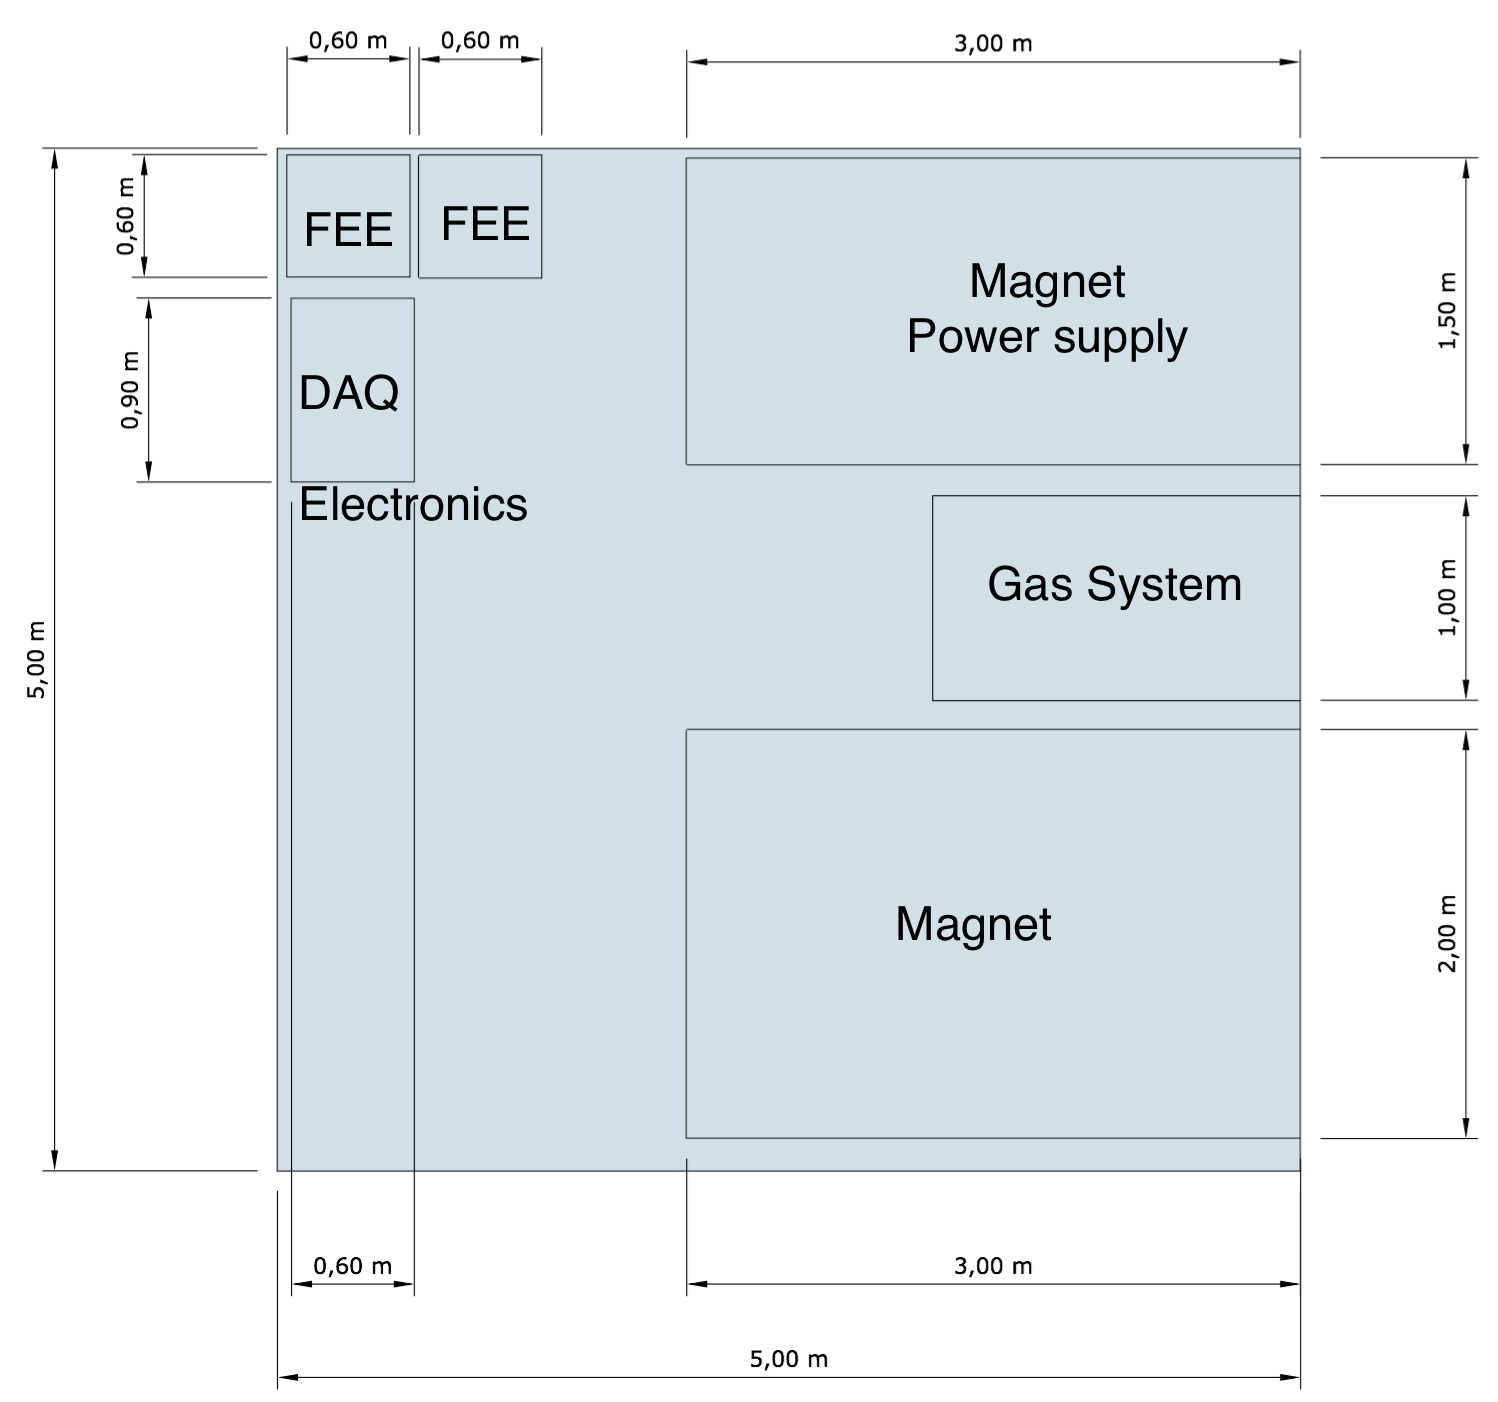
\includegraphics[width=\textwidth]{img/distribution2.png}
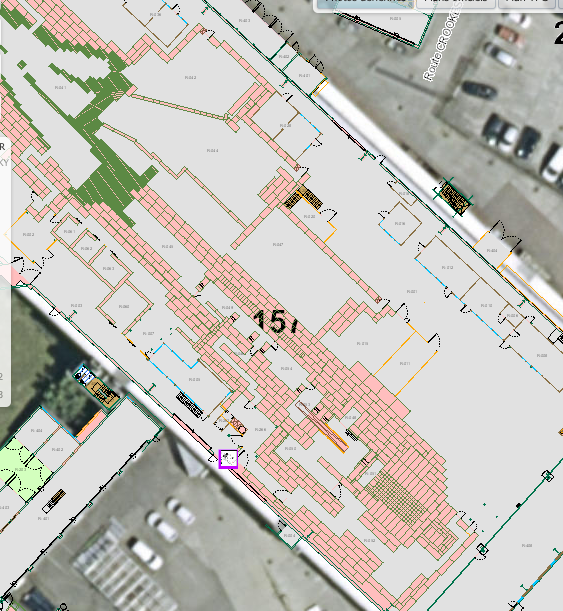
\includegraphics[angle=0,width=\textwidth]{img/generalmap.png}
\caption{Location of the experimental area} \label{fig:location}
\end{figure}


\begin{figure}
\centering
%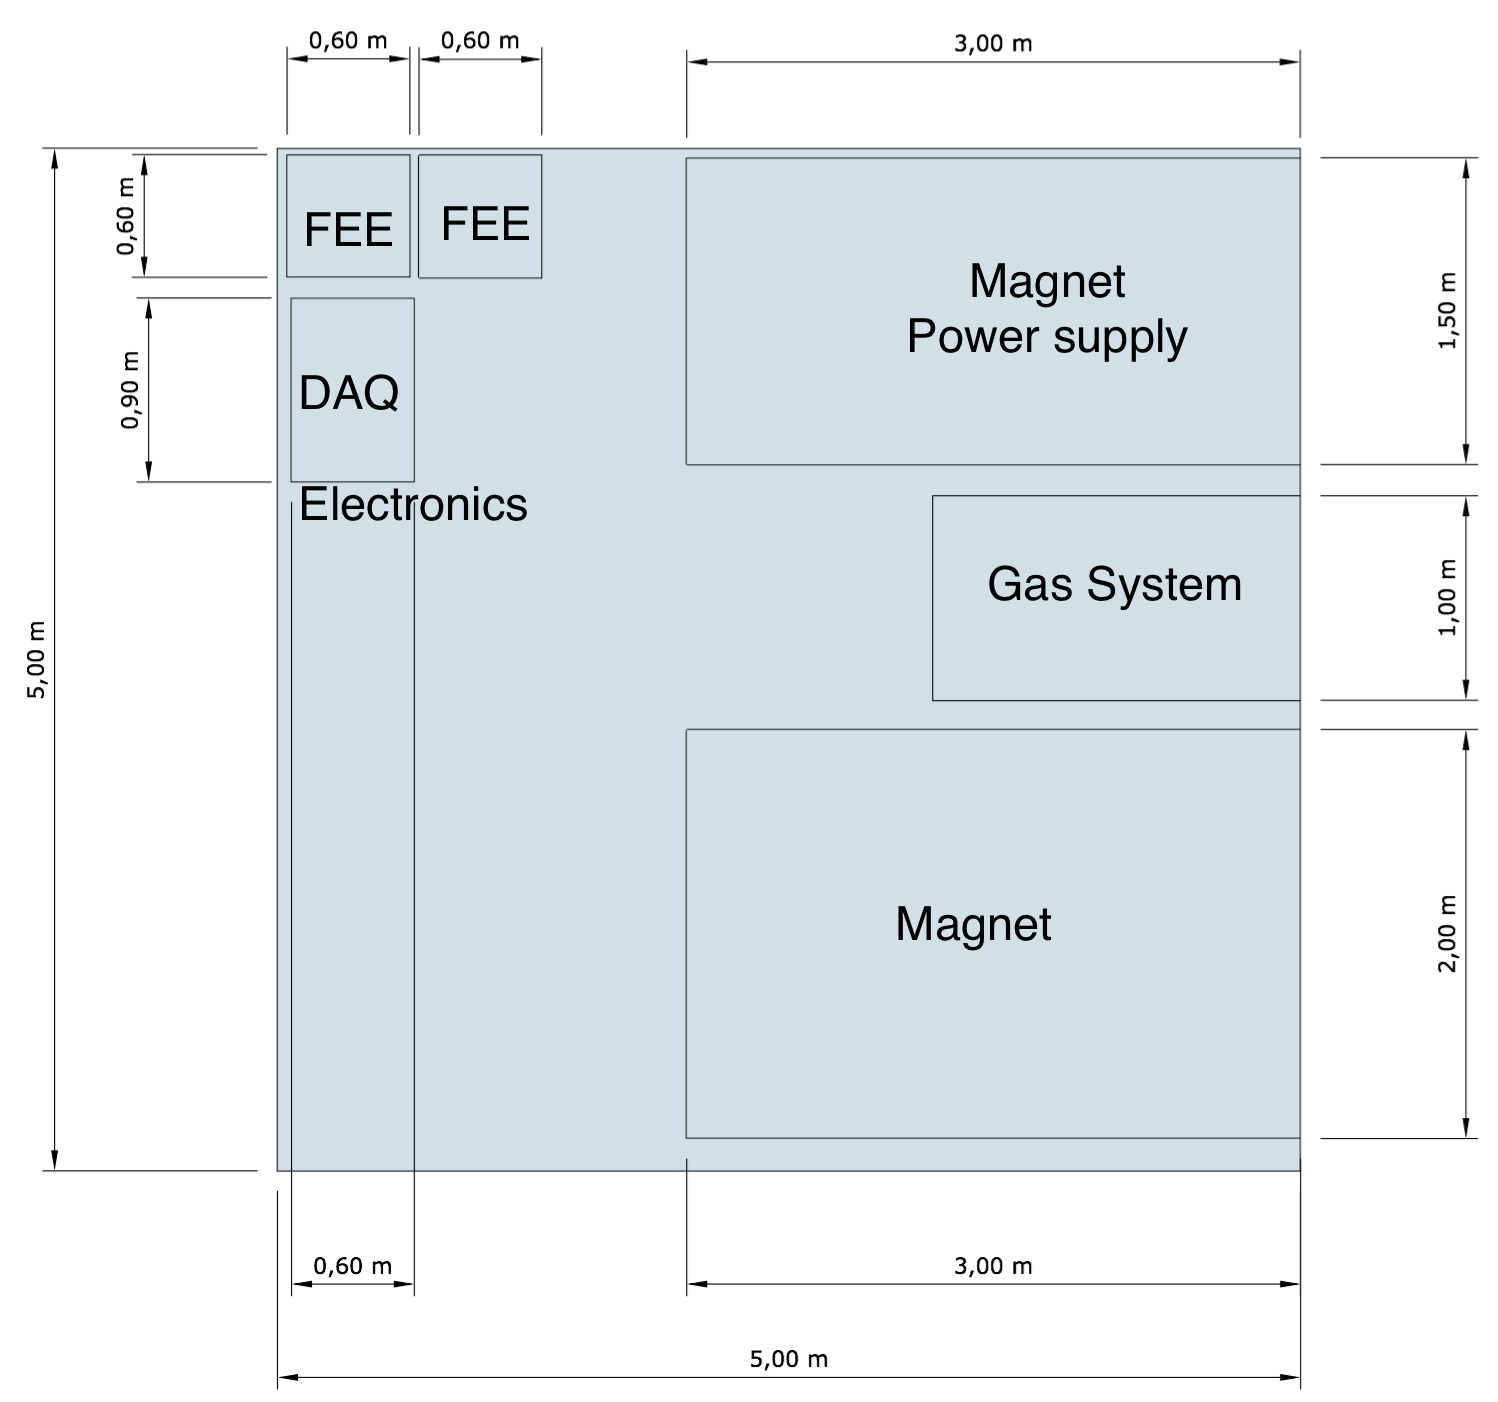
\includegraphics[width=\textwidth]{img/distribution2.png}
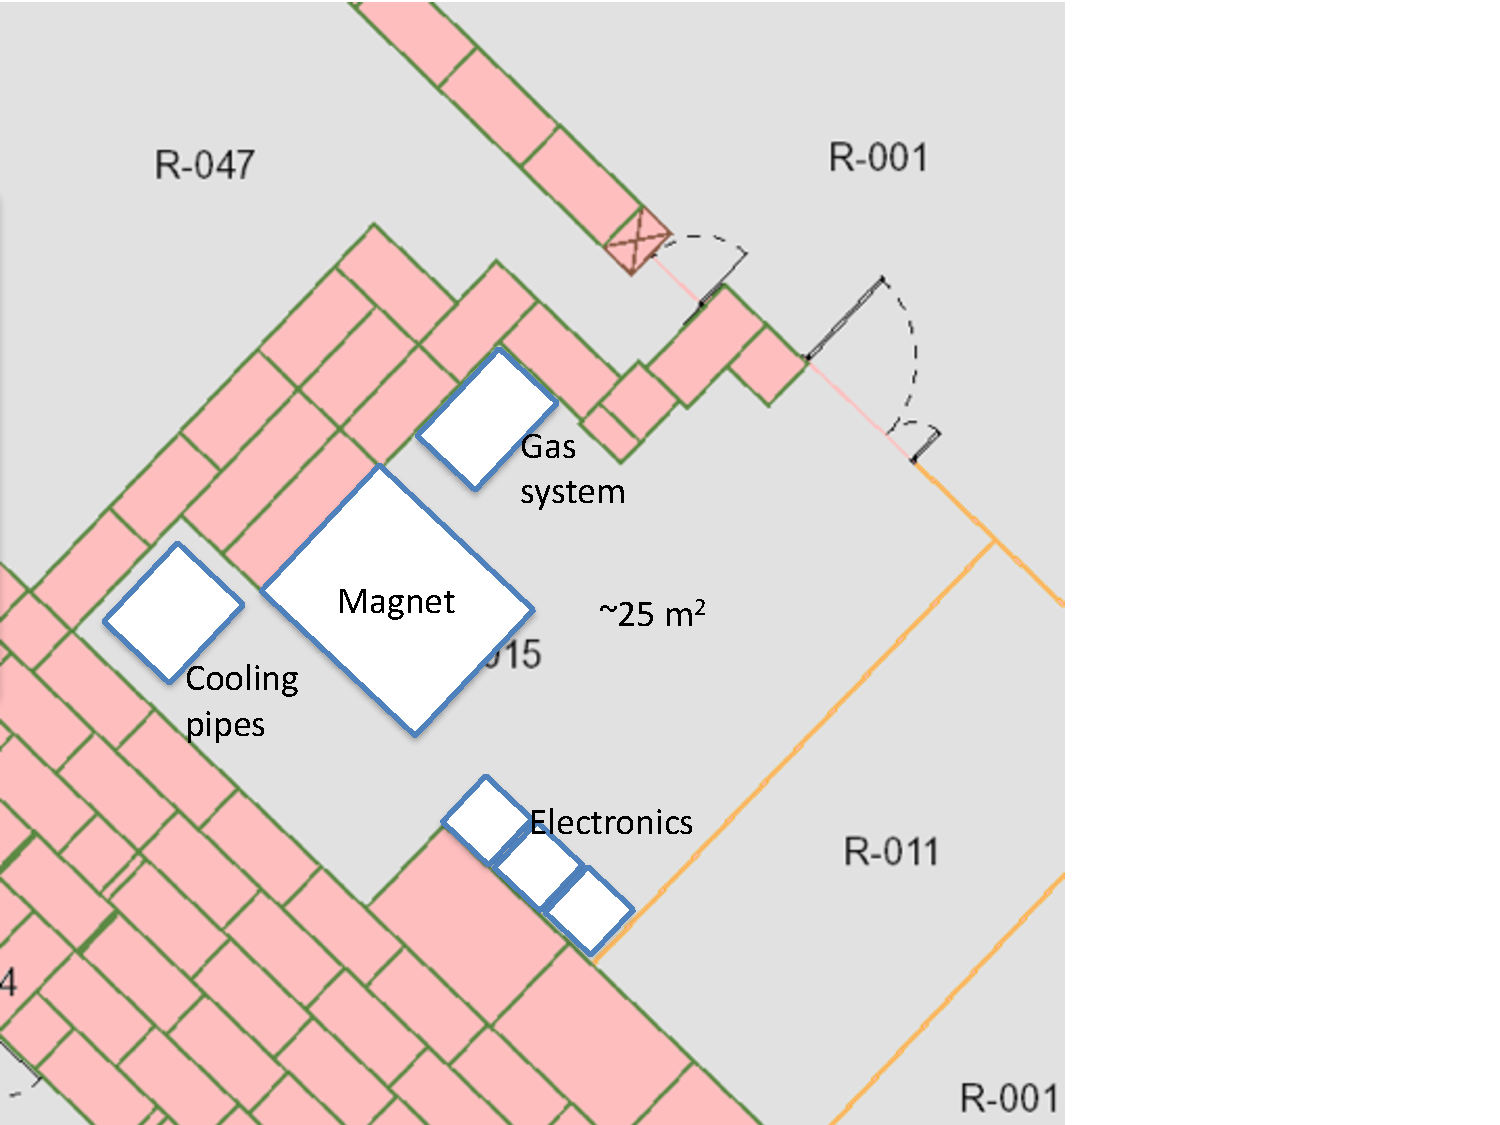
\includegraphics[angle=0,width=\textwidth]{img/distribution_examples.pdf}
\caption{Proposed distribution of the NEXT-DEMO, magnet and all different necessary systems for the operation of the detector in the experimental area} \label{fig:Distribution2}
\end{figure}


\begin{figure}
\centering
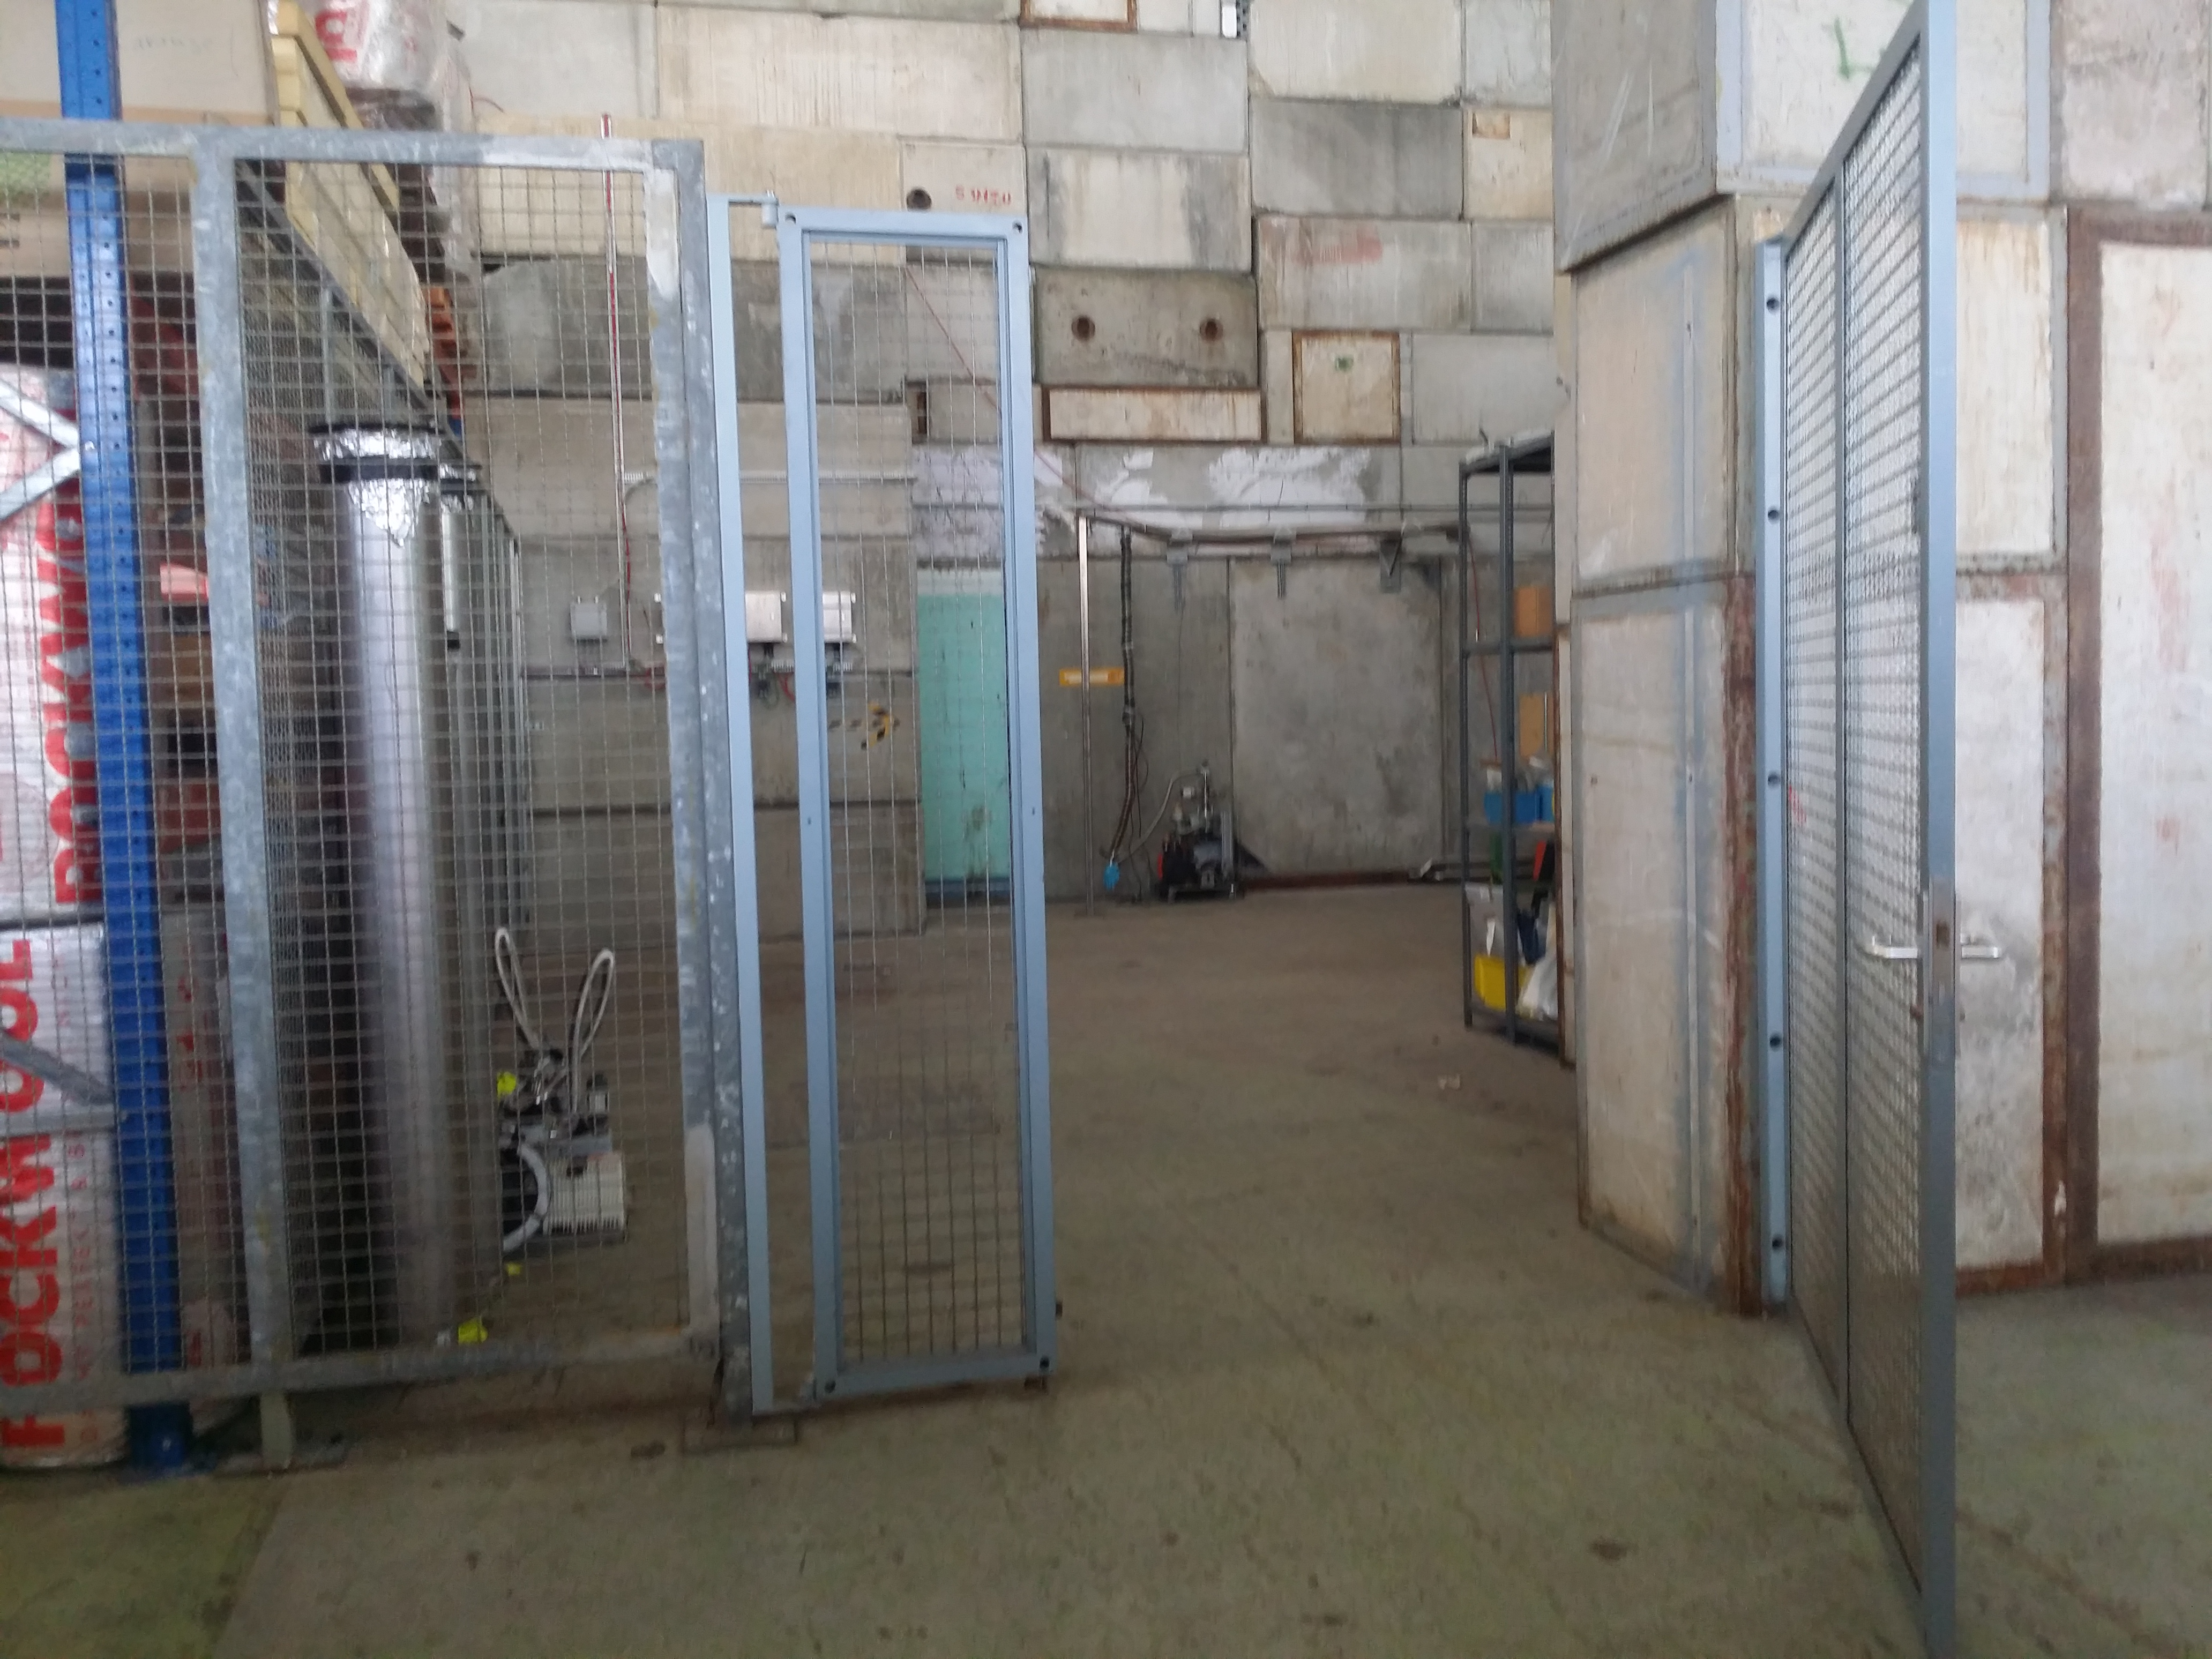
\includegraphics[width=0.45\textwidth]{img/experimentalarea1.jpeg}
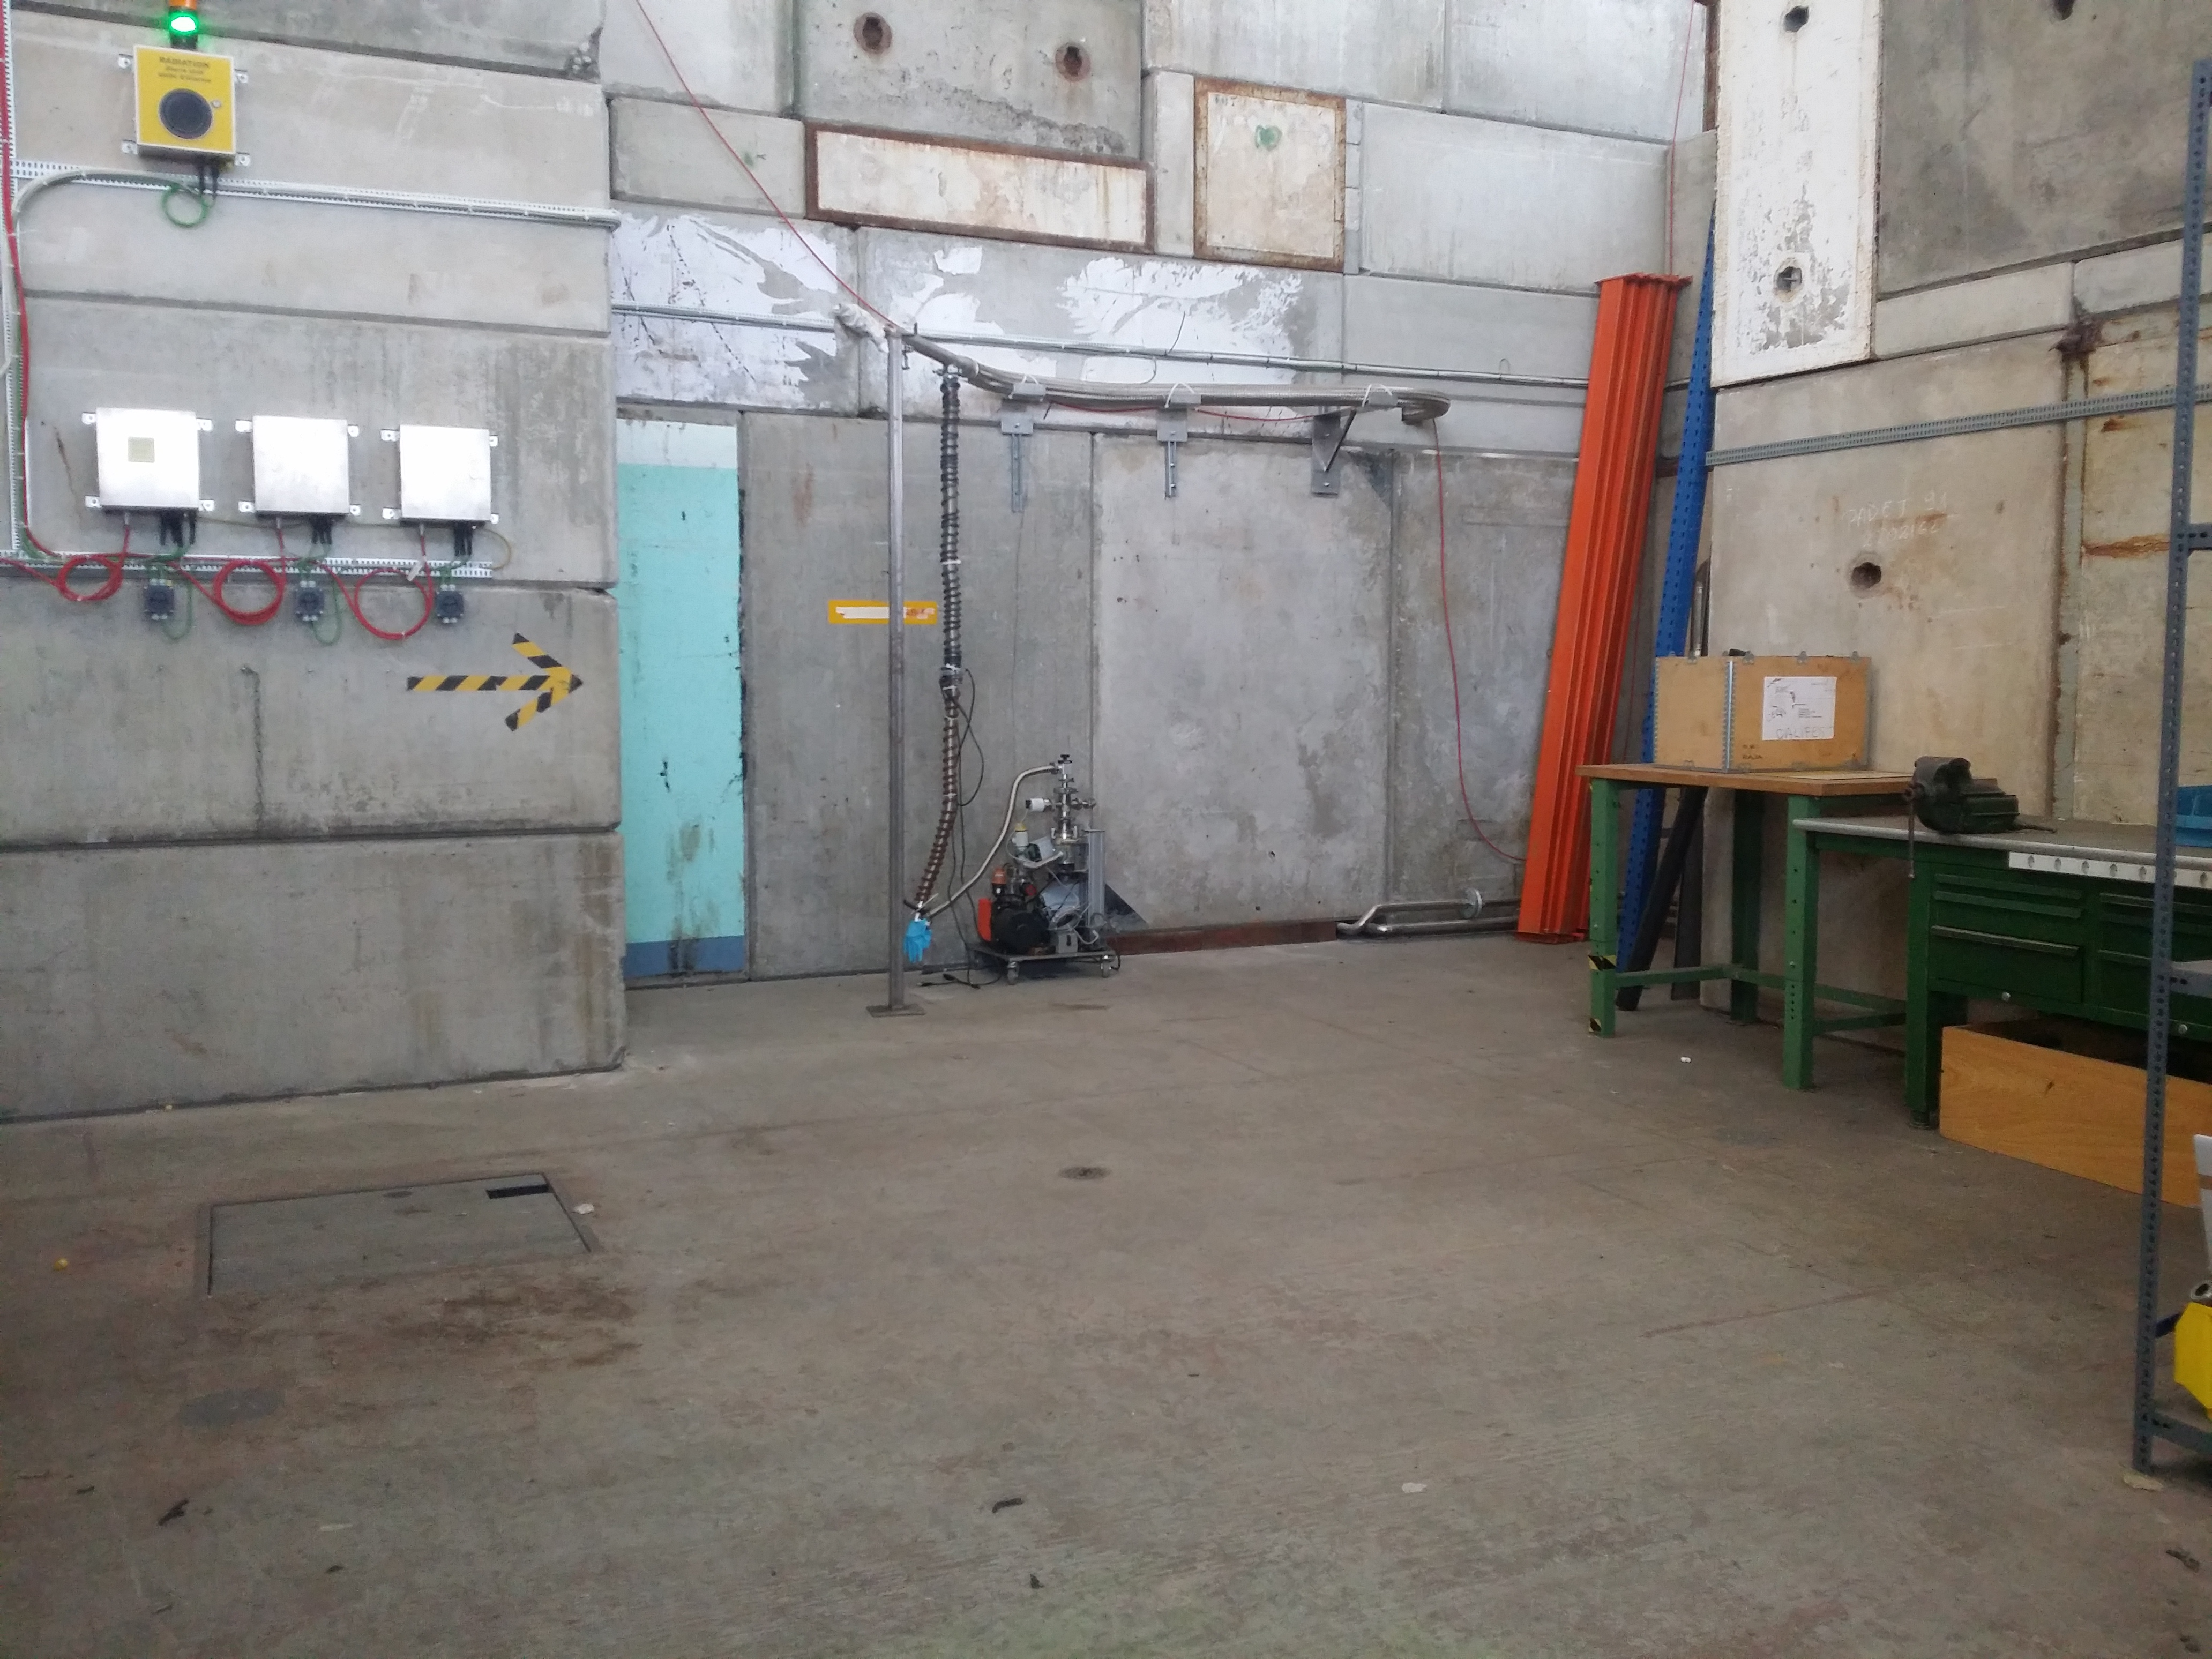
\includegraphics[angle=0,width=0.45\textwidth]{img/experimentalarea2.jpeg}
\caption{Proposed distribution of the NEXT-DEMO, magnet and all different necessary systems for the operation of the detector in the experimental area} \label{fig:pictures}
\end{figure}


\subsection{Related Gas systems}

Only one gas system will be used in the area. The gas system has been described in the main document. The following table summarizes the quantity and distribution of the different gases to be used in NEXT-DEMO:



\begin{table}[h]
%\resizebox{1.4\textwidth}{!}{\begin{minipage}{\textwidth}
\begin{tabular}{|r|r|r|r|r|}
\hline
\parbox[t]{2cm}{Gas Type} & \parbox[t]{3cm}{Supply description} &\parbox[t]{3cm}{ Volume (gas at ambient P ad T) }& \parbox[t]{3cm}{Supply location (see figure \ref{fig:Distribution2}) }& Comments \\\hline
Xenon & One bottle & 255 liters & GS 1 & \\\hline
CO2 & One bottle & 200 liters (approx.) & GS 1 &\\\hline
\end{tabular}
\caption{Gas supply for NEXT-DEMO}
\label{tab:gassupply}
%\end{minipage} }
\end{table}

\subsection{Gas release risk assesment}

\subsubsection{Relevant Facts}
\begin{itemize}
\item All gases are at room temperature during normal operation.
\item A gas leak of the order of 1\% is easily detected.
\item All used gases are transparent and odorless.
\end{itemize}

\subsubsection{Risk assesment}

\textit{Scenario 1}

A leak due to a material breaking of a material impact that causes a hole with a size of the a 1/4" in the gas system. Total loss of the gas. 

\textbf{Consequences:} The total volume will around 15 minutes for a complete release to the atmosphere. The total volume of Xenon is described in the \textbf{Safety} section of this document. The drop of pressure will be detected by the slow control system and it will stop the pump. People should leave the area until the pressure reaches a stable level in all different pressure gauges.

\textit{Scenario 2}
 
 A leak occurs during cryogenic recovery of the Xenon. 
 
 \textbf{Consequences:} In this case the slow control will be innactivated. In the other hand, most of the Xenon should be frozen and the total volume of Xenon released to the atmosphere won't be relevant.
 

\subsection{Conclusions}

\subsubsection{Oxygen detection hazard}

Takin in consideration all possible risks and the mitigation actions, it is recommended to install Oxygen Detection Heads.

Local flashing lights inside the area as well as at each entry can be installed and connected to the slow control if necessary.

